\documentclass[spanish,xcolor=table]{beamer}
\usepackage[spanish]{babel}
\selectlanguage{spanish}
\usepackage[utf8]{inputenc}
\mode<presentation> {

%----------------Beamer Themes--------------------

\usetheme{Boadilla}

%--------------------Beamer Font & Colors----------

\usecolortheme{seahorse}

%-------------------Beamer Options --------------------

\setbeamertemplate{navigation symbols}{} % To add the navigation symbols from the bottom of all slides comment this line
}

%-------------------Package----------------------------
\RequirePackage{natbib}
\usepackage{graphicx} 
\usepackage{booktabs} % use of \toprule, \midrule and \bottomrule in tables
\usepackage{tikz}
\usepackage{pgfplots}
\usepackage{multirow}
\usepackage{multicol}
\usepackage{amsmath}
\usepackage{hhline}
\usepackage[export]{adjustbox} %para posicionar imagenes(ej, left, right)

%---Librerias de Tikz -----------------------------
\usetikzlibrary{arrows,calc}
\usetikzlibrary{intersections}
\usetikzlibrary{pgfplots.fillbetween}
\usetikzlibrary{patterns}
\usetikzlibrary{plotmarks}
\usetikzlibrary{calc}
\usetikzlibrary{matrix}
\usetikzlibrary{positioning}
\usepackage{relsize}
\usepackage[nointegrals]{wasysym}
\usepackage{caption}
\usepackage{bigints}
\usepackage{xcolor}
%---------------------------------------------------------------------------------

%-----------Tikz Layers---------------------------------
\pgfdeclarelayer{ft}
\pgfdeclarelayer{bg}
\pgfsetlayers{bg,main,ft}
%---------------------------------------------------------


%--------Definiciones de Operadores --------------
\DeclareMathOperator*{\argmax}{arg\,max}
\def\checkmarkt{\tikz\fill[scale=0.4](0,.35) -- (.25,0) -- (1,.7) -- (.25,.15) -- cycle;} 
\newcommand{\bigqm}[1][1]{\text{\larger[#1]{\textbf{?}}}}
\let\Tiny=\tiny % fix issue font name beamer
\makeatletter

\newcommand\mathcircled[1]{%
  \mathpalette\@mathcircled{#1}%
}
\newcommand\@mathcircled[2]{%
  \tikz[baseline=(math.base)] \node[draw,circle,inner sep=1pt] (math) {$\m@th#1#2$};%
}

%north west lines pattern density ajusted
\pgfdeclarepatternformonly[\LineSpace,\LineSpaceColor]{MNWL}{\pgfqpoint{-1pt}{-1pt}}{\pgfqpoint{\LineSpace}{\LineSpace}}{\pgfqpoint{\LineSpace}{\LineSpace}}%
{
    \pgfsetcolor{\tikz@pattern@color}
    \pgfsetlinewidth{0.4pt}
    \pgfpathmoveto{\pgfqpoint{0pt}{\LineSpace}}
    \pgfpathlineto{\pgfqpoint{\LineSpace + 0.1pt}{-0.1pt}}
    \pgfsetstrokecolor{\LineSpaceColor}%        % <-- added
    \pgfusepath{stroke}
}
\makeatother

\newdimen\LineSpace
\tikzset{
    line space/.code={\LineSpace=#1},
    line space=6pt, %this ajust density of MNWL
    line color/.store in=\LineSpaceColor,      % <-- added
    line color=black,
} %line set color in custom parttern check line 665-667 for an example

%----------------------------------------------------------------------------------------
%	           Slide Inicial
%----------------------------------------------------------------------------------------
 

\title[ECO -TS101]{Econometr\'\i{}a de Series de Tiempo} 
\subtitle{T\'opico VI - Introduction to Neural Networks}

%Profesores

\author{Marcelo Villena Ch., PhD} 

%-----------------------------------------------------------------

\institute[UAI] % Your institution as it will appear on the bottom of every slide, may be shorthand to save space
{
Universidad Adolfo Ib\'a\~nez 
 \\ % institution for the title page
\medskip
}
\date{} % Date, can be changed to a custom date

%-------------------Figure Settings-------------------
\pgfplotsset{ % Here we specify options for all figures in the document
  compat=1.8, % Which version of pgfplots do we want to use?
  legend style = {font=\small\sffamily}, % Legends in a sans-serif font
  label style = {font=\small\sffamily} % Labels in a sans-serif font
}

%-----Color definitions-------------
\colorlet{ColorG}{black!60!green}
\colorlet{ColorR}{black!60!red}
\colorlet{ColorB}{black!60!blue}
\colorlet{ColorY}{black!40!yellow}
%-----------------------------------

\begin{document}

\begin{frame}

\begin{figure}[t!]

\includegraphics[scale=0.1]{Logo.jpg}
\end{figure}
\titlepage % Print the title page as the first slide
\end{frame}

\begin{frame}
\frametitle{Contenidos} 
\tableofcontents % Lista de contenidos, carga la instruccion \section{} y \subsection{} 
\end{frame}


%----------------------------------------------------------------------------------------
%	PRESENTATION SLIDES
%----------------------------------------------------------------------------------------

%------------Slides------------------------------------
%---------------------Slide 3--------------------------
\begin{section}{Introduci\'on a las Redes Neuronales}
\begin{frame}
\frametitle{Introduci\'on a las Redes Neuronales}

Un tema popular en el an\'alisis de datos moderno es la red neuronal, el cual se puede clasificar como un m\'etodo semiparam\'etrico. La literatura sobre redes neuronales es enorme, y su aplicaci\'on se extiende a muchas \'areas cient\'{\i}ficas con diversos grados de \'exito. \cite{cheng1994neural} proporcionan informaci\'on sobre redes neuronales desde un punto de vista estad\'{\i}stico. \\
Primeramente, nos enfocaremos en las redes neuronales feed-forward (Feed forward neural network) en las cuales las entradas est\'an conectadas a una o m\'as neuronas, o nodos, en la capa de entrada, y estos nodos est\'an conectados a otras capas hasta que alcanzan la capa de salida. 

\end{frame}
%---------------------------------------------------------
%---------------------Slide 4--------------------------
\begin{frame}
\frametitle{Introduci\'on a las Redes Neuronales}
Las redes neuronales son un marco de aprendizaje autom\'atico (machine learning framework), que intenta imitar el patr\'on de aprendizaje de las redes neuronales biol\'ogicas naturales. Las redes neuronales biol\'ogicas tienen neuronas interconectadas con dendritas que reciben entradas, y luego, basadas en estas entradas, producen una senal de salida a trav\'es de un ax\'on a otra neurona. Tratamos de imitar este proceso mediante el uso de Redes neuronales artificiales (Artificial neuronal networks ANN), que a partir de ahora llamaremos redes neuronales. El proceso de crear una red neuronal comienza con la forma m\'as b\'asica, un s\'olo perceptr\'on.
\end{frame}
%---------------------------------------------------------
%---------------------Slide 5--------------------------
\begin{frame}
\frametitle{Introduci\'on a las Redes Neuronales}

Posteriormente, introduciremos las Support Vector Machine (SVM).  En el aprendizaje autom\'atico (machine learning), los Support Vector Machine (SVM) son modelos de aprendizaje supervisados mediante algoritmos que permiten analizar los datos utilizados para la clasificaci\'on y el an\'alisis de regresi\'on.\\
En particular, dado un conjunto de ejemplos de entrenamiento, cada uno marcado como perteneciente a una u otra de dos categor\'{i}as, un algoritmo de entrenamiento SVM construye un modelo que asigna nuevos datos a una de las dos categor\'{i}as, convirti\'endolo en un clasificador lineal binario no probabil\'{i}stico.\\
 Un modelo SVM es una representaci\'on de los datos como puntos en el espacio, mapeados de manera que los ejemplos de las categor\'{i}as, est\'an divididas por un espacio libre lo m\'as ancho posible. A continuaci\'on, se mapean nuevos datos en ese mismo espacio y se predice que pertenecen a una categor\'{i}a seg\'un el lado del espacio en el que caen.

\end{frame}
\end{section}
%---------------------------------------------------------
%---------------------Slide 6--------------------------
\begin{section}{Feed forward neural network}
\begin{frame}
\frametitle{Feed forward neural network}

Desarrollaremos un ejemplo de una red de feed-forward simple para an\'alisis de series temporales univariadas con una capa oculta. La capa de entrada tiene dos nodos, y la capa oculta tiene tres. Los nodos de entrada se conectan hacia adelante a todos y cada uno de los nodos de la capa oculta, y estos nodos ocultos se conectan al \'unico nodo en la capa de salida. Llamamos a la red una red de feed-forward.\\
Las redes neuronales m\'as complicadas, incluidas las que tienen conexiones de retroalimentaci\'on, han proliferado, pero las redes de feed-forward son las m\'as relevantes para nuestro estudio.

\end{frame}
%---------------------------------------------------------
%---------------------Slide 7--------------------------
\begin{frame}
\frametitle{Feed forward neural network}

Una red neuronal feed-forward con una capa oculta para el an\'alisis de series temporales univariadas.

\begin{figure}[t!]
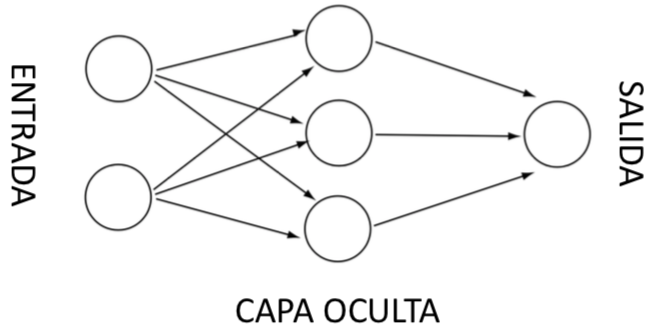
\includegraphics[scale=0.3]{NN.pdf}
\end{figure}
 
\end{frame}

%---------------------------------------------------------
%---------------------Slide 8--------------------------
\begin{frame}
\frametitle{Feed forward neural network}

El perceptr\'on recibe entradas, las multiplica por un poco de peso y luego las pasa a una funci\'on de activaci\'on para producir una salida. Es as\'{i} como, una red neuronal procesa informaci\'on de una capa a la siguiente mediante una "funci\'on de activaci\'on". Considere una red de feed-forward con una capa oculta. El j-\'esimo nodo en la capa oculta se define como

\begin{equation} 
h_j = f_j \left(\alpha_0j + \sum_{i \to j} w_ij x_i \right)
\end{equation}

donde $x_i$ es el valor del i-\'esimo nodo de entrada, $f_j (.)$ es una funci\'on de activaci\'on que generalmente se toma como la funci\'on log\'{\i}stica:

\begin{equation*} 
f_j (z) = \frac{exp(z)}{1+exp(z)'}
\end{equation*}

$\alpha_{0 j}$ se llama sesgo, la suma $i \to j$ significa sumando todos los nodos de entrada que alimentan a $j$, y $w_{ij}$ son los pesos.

\end{frame}
%---------------------------------------------------------
%---------------------Slide 9--------------------------
\begin{frame}
\frametitle{Feed forward neural network}

A modo ilustrativo, el j-i\'esimo nodo de la capa oculta de la red de avance 2-3-1 en la figura es:
\begin{equation}   \label{eq:-1}
h_j = \frac{exp(\alpha_{0j}+w_{1j} x_1+w_{2j} x_2)}{1+\alpha_0j+w_{1j} x_1+w_{2j} x_2)}, j=1,2,3.
\end{equation}

Para la capa de salida, el nodo se define como:

\begin{equation} 
o = f_o \left(\alpha_{0o} + \sum_{j \to o} w_{jo} h_j \right)
\end{equation}

donde la funci\'on de activaci\'on $f_o (.)$ es lineal o una funci\'on de escal\'on unitario (Heaviside function). Si $f_o (.)$ es lineal, entonces:

\end{frame}
%---------------------------------------------------------
%---------------------Slide 10--------------------------
\begin{frame}
\frametitle{Feed forward neural network}

\begin{equation*} 
o =  \alpha_{0o} + \sum_{j \to o} w_{jo} h_j 
\end{equation*}

donde $k$ es la cantidad de nodos en la capa oculta. Por una funci\'on  de escal\'on unitario, queremos decir $f_o(z)=1$ si $z > 0$ y $f_o(z)=0$  en caso contrario. Una neurona con una funci\'on de escal\'on unitario se llama neurona umbral, con "1" que indica que la neurona env\'{\i}a su mensaje. Por ejemplo, la salida de la red 2-3-1 en la figura es:
\begin{equation*} 
o = \alpha_{0o}+w_{1o} h_1+w_{2o} h_2+w_{3o} h_3
\end{equation*}
\end{frame}
%---------------------------------------------------------
%---------------------Slide 11--------------------------
\begin{frame}
\frametitle{Feed forward neural network}

Si la funci\'on de activaci\'on es lineal, tenemos:

\begin{equation*}
  o=\begin{cases}
    1, & \text{if $\alpha_{0o}+w_{1o} h_1+w_{2o} h_2+w_{3o} h_3>0$}.\\
    0, & \text{if $\alpha_{0o}+w_{1o} h_1+w_{2o} h_2+w_{3o} h_3 \leq 0$}.
  \end{cases}
\end{equation*}
Si  $f_o (.)$ es una funci\'on de escal\'on unitario.

Al combinar las capas, la salida de una red neuronal feed-forward se puede escribir como:
\begin{equation} \label{eq:1}
o = f_0 \left[ \alpha_{0o} + \sum_{j \to o} w_{jo} f_j \left( \alpha_{0j} + \sum_{i \to j} w_{ij} x_i \right) \right]
\end{equation}

\end{frame}
%---------------------------------------------------------
%---------------------Slide 12--------------------------
\begin{frame}
\frametitle{Feed forward neural network}

Si uno tambi\'en permite conexiones directas desde la capa de entrada a la capa de salida, entonces la red se convierte en:
\begin{equation}  \label{eq:2}
o = f_0 \left[ \alpha_{0o} + \sum_{i \to o} \alpha_{io} x_i + \sum_{j \to o} w_{jo} f_j \left( \alpha_{0j} + \sum_{i \to j} w_{ij} x_i \right) \right]
\end{equation}

donde la primera suma se suma a los nodos de entrada. Cuando la funci\'on de activaci\'on de la capa de salida es lineal, las conexiones directas desde los nodos de entrada al nodo de salida representan una funci\'on lineal entre las entradas y la salida. En consecuencia, en este caso particular, el modelo presentado en la ecuaci\'on \ref{eq:2}, es una generalizaci\'on de modelos lineales. Para la red 2-3-1 de nuestra figura, si la funci\'on de activaci\'on de salida es lineal, entonces la ecuaci\'on \ref{eq:1} se convierte en:

\begin{equation*} 
o =  \alpha_{0o} + \sum_{j=1}^ {3} w_{jo} h_j 
\end{equation*}
donde $h_j$ se obtiene de la ecuaci\'on \ref{eq:-1}.
\end{frame}
%---------------------------------------------------------
%---------------------Slide 13--------------------------
\begin{frame}
\frametitle{Feed forward neural network}

 La red tiene 13 par\'ametros. Si utilizamos la ecuaci\'on \ref{eq:2},  la red se convierte en:
\begin{equation*} 
o =  \alpha_{0o} + \sum_{i=1}^ {2}  \alpha_{io} x_i  + \sum_{j=1}^ {3} w_{jo} h_j 
\end{equation*}
donde $h_j$ se obtiene de la ecuaci\'on \ref{eq:-1}. El n\'umero de par\'ametros de la red aumenta a 15.
\end{frame}
%---------------------------------------------------------
%---------------------Slide 14--------------------------
\begin{frame}
\frametitle{Feed forward neural network}

Nos referimos a la funci\'on en la ecuaci\'on \ref{eq:1} o \ref{eq:2} como una funci\'on semiparami\'etrica porque se conoce su forma funcional, pero se desconoce el n\'umero de nodos y sus desviaciones y pesos.\\
Las conexiones directas desde la capa de entrada a la capa de salida en la ecuaci\'on \ref{eq:2}, significa que la red puede omitir la capa oculta. Nos referimos a dicha red como una red de feed-forward de capa de salto.\\
Las redes feed-forward se conocen como percentrones multicapa en la literatura de redes neuronales. Pueden aproximar cualquier funci\'on continua uniformemente en conjuntos compactos aumentando la cantidad de nodos en la capa oculta, ver \cite{hornik1989multilayer}, \cite{chen1995universal}. Esta propiedad de las redes neuronales es la propiedad de aproximaci\'on universal de los percetrones multicapa. \\
\textbf{En resumen, las redes neuronales feed-forward con una capa oculta se pueden ver como una forma de parametrizar una funci\'on no lineal continua general.}

\end{frame}
%---------------------------------------------------------
%---------------------Slide 15--------------------------
\begin{frame}
\frametitle{Feed forward neural network}

\textbf{Training and Forecasting}

La aplicaci\'on de redes neuronales implica dos pasos. \\
El primer paso es entrenar (training) a la red (es decir, para construir una red, incluida la determinaci\'on del n\'umero de nodos y la estimaci\'on de sus sesgos y ponderaciones). \\
El segundo paso es la inferencia, especialmente el pron\'ostico extra-muestral (forecasting).\\
Al comparar el resultado comparado de cada pron\'ostico, se selecciona la red que supera a las dem\'as, defini\'edose como la mejor red para realizar inferencias. 
\end{frame}
%---------------------------------------------------------
%---------------------Slide 16--------------------------
\begin{frame}
\frametitle{Feed forward neural network}
\textbf{Training and Forecasting}
En una aplicaci\'on de serie de tiempo, supongamos que $\{(r_t, x_t) | t = 1, ..., T\}$ representan los datos disponibles para el entrenamiento de la red, donde $x_t$ denota el vector de entradas, y $r_t$ es la serie de inter\'es (por ejemplo, retornos-log de un activo). \\
Para una red determinada, supongamos que $o_t$ sea la salida de la red, con una entrada de $x_t$; ver el modelo presentado en la ecuaci\'on \ref{eq:2}. \\
El entrenamiento de una red neuronal equivale a elegir sus sesgos y pesos de forma de minimizar algunos criterios de ajuste, por ejemplo, el m\'{\i}nimo cuadrado de su error\\
\begin{equation*} 
S^2 =  \sum_{t=1}^ {T}  (r_t - o_t)^2 
\end{equation*}
\end{frame}
%---------------------------------------------------------
%---------------------Slide 17--------------------------
\begin{frame}
\frametitle{Feed forward neural network}
\textbf{Training and Forecasting}

Este es un problema de estimaci\'on no lineal que puede ser resuelto por varios m\'etodos iterativos. Para garantizar la continuidad (smoothness) de la funci\'on ajustada, se pueden agregar algunas restricciones adicionales al problema de minimizaci\'on anterior. \\
En la literatura de redes neuronales, el algoritmo de aprendizaje Back Propagation (BP) es el m\'etodo m\'as popular para el entrenamiento de una red. El m\'etodo BP, introducido por \cite{bryson1969applied}, funciona hacia atr\'as comenzando con la capa de salida, y usa una regla de gradiente (gradient rule) para modificar los sesgos y los pesos iterativamente.\\
 Una vez que se construye una red neuronal feed-forward, se puede usar para calcular pron\'osticos extramuestrales.
\end{frame}
%---------------------------------------------------------
%---------------------Slide 18--------------------------
\begin{frame}
\frametitle{Feed forward neural network}
\textbf{Training and Forecasting}

En resumen, una vez que tenemos la salida, podemos compararla con una serie conocida y ajustar los pesos de la mejor forma posible (los pesos usualmente comienzan con valores de inicializaci\'on aleatorios). Seguimos repitiendo este proceso hasta que hayamos alcanzado un n\'umero m\'aximo de iteraciones permitidas, o una tasa de error aceptable.\\
Para crear una red neuronal, simplemente comenzamos a agregar capas de perceptrones, creando un modelo de perceptr\'on multicapa de una red neuronal. Tendremos una capa de entrada que tomar\'a directamente las entradas de funciones y una capa de salida que crear\'a las salidas resultantes. Las capas intermedias se conocen como capas ocultas porque no ven directamente las entradas o salidas de caracter\'{i}sticas

\end{frame}
%---------------------------------------------------------
%---------------------Slide 19--------------------------
\begin{frame}
\frametitle{Feed forward neural network}
\textbf{Pre-procesamiento de datos}

Es importante normalizar los datos antes de entrenar una red neuronal. La red neuronal puede tener dificultades para converger antes de la cantidad m\'axima de iteraciones permitidas si los datos no están normalizados. Hay muchos m\'etodos diferentes para la normalizaci\'on de datos. Por lo general, es mejor escalar los datos de 0 a 1, o de -1 a 1. 

\end{frame}
%---------------------------------------------------------
%---------------------Slide 20--------------------------
\begin{frame}
\frametitle{Feed forward neural network}
\textbf{Ejemplo 1} 

Para ilustrar las potenciales aplicaciones de redes neuronales en finanzas, modelaremos los retornos mensuales, incluyendo dividendos, de la firma IBM de enero de 1926 a diciembre de 1999. \\
Dividimos los datos en dos sub-muestras. La primera sub-muestra, que consiste en retornos de enero de 1926 a diciembre de 1997 para 864 observaciones, se usa para modelar. \\
Usando el modelo presentado en la ecuaci\'on \ref{eq:2}, con tres entradas y dos nodos en la capa oculta, obtenemos una red 3-2-1 para la serie. Las tres entradas son $r_{t-1}$, $r_{t-2}$ y $r_{t-3}$, y los sesgos y ponderaciones se presentan a continuaci\'on:

\begin{equation*} 
r_t = 3.22 - 1.81 f_1 (r_{t-1}) - 2.28 f_2 (r_{t-1}) - 0.09 r_{t-1} - 0.05r_{t-2} - 0.12r_{t-3} 
\end{equation*}

donde, $r_{t-1} = (r_{t-1},r_{t-2},r_{t-3})$ 
\end{equation*}

\end{frame}
%---------------------------------------------------------
%---------------------Slide 21--------------------------
\begin{frame}
\frametitle{Feed forward neural network}

y las dos funciones log\'{\i}sticas son:

\begin{equation*} 
f_1(r_{t-1}) = \frac { exp (-8.34 -18.97r_{t-1} + 2.17 r_{t-2} -19.17 r_{t-3})}{1 + exp(-8.34 -18.97r_{t-1} + 2.17 r_{t-2} -19.17 r_{t-3})}  
\end{equation*}

\begin{equation*} 
f_2(r_{t-1}) = \frac { exp (39.25 -22.17 r_{t-1} - 17.34 r_{t-2} -5.98 r_{t-3})}{1 + exp (39.25 -22.17 r_{t-1} - 17.34 r_{t-2} -5.98 r_{t-3})}  
\end{equation*}

El error est\'andar de los residuos para el modelo anterior es 6.56. Para comparaci\'on, tambi\'en construy\'o un modelo AR para los datos, obteni\'endose el siguente modelo:\\
\begin{equation*}
r_t = 1.101 + 0.077r_{t -1} + a_t
\end{equation*}
con $\sigma_a = 6.61$\\
El error est\'andar residual es ligeramente mayor que el del modelo feed-forward.
\end{frame}
%---------------------------------------------------------
%---------------------Slide 22--------------------------
\begin{frame}
\frametitle{Feed forward neural network}
\textbf{Comparaci\'on de Pron\'ostico}
Las rentabilidades mensuales de las acciones de IBM en 1998 y 1999 forman la segunda submuestra y se utilizan para evaluar el rendimiento de las predicciones fuera de muestra de las redes neuronales.\\
Como punto de referencia para la comparaci\'on, utilizamos la media muestral de $r_t$ en la primera submuestra como el pron\'ostico de 1 paso para todas las rentabilidades mensuales en la segunda submuestra. Esto equivale a suponer que el precio mensual del precio de las acciones de IBM sigue una caminata aleatoria con drift.\\ 
El error de pron\'ostico cuadr\'atico medio (MSE) del modelo de referencia es 91.85. Para el modelo AR (1), el MSE de los pron\'osticos de 1 paso adelante es 91.70. Por lo tanto, el modelo AR (1) supera ligeramente al benchmark. Para la red, el MSE es 91.74.
\end{frame}
%---------------------------------------------------------
%---------------------Slide 23--------------------------
\begin{frame}
\frametitle{Feed forward neural network}
\textbf{Ejemplo 2 - Pronosticando el S$&$P 500} 

\vspace{4mm}	

En el presente ejemplo pronosticaremos el S$&$P 500 usando modelos univariados. 
En particular, usaremos un modelo lineal, como es el ARIMA, y uno no-lineal, una feed-forward neural network.

\vspace{4mm}	

\only<1|handout:1>{
\begin{exampleblock}{C\'odigo en R}

library(neuralnet)\\
library(nnet)\\
library(forecast)\\

getSymbols(``SPY", from = ``2000-01-01", to = ``2017-12-01", src =  ``yahoo", adjust =  TRUE, periodicity = ``monthly")\\
Returns = diff(log(Ad(SPY)))\\
Returns[as.character(head(index(Ad(SPY)),1))] = 0\\

\end{exampleblock}
}

\end{frame}

%---------------------------------------------------------
%---------------------Slide 24--------------------------
\begin{frame}
\frametitle{Feed forward neural network}
\textbf{Ejemplo 2 - Pronosticando el S$&$P} 
\vspace{4mm}	

\textbf{nnetar (Neural Network Time Series Forecast)} es una red neuronal del tipo feed-forward que considera valores rezagados de ``y” como entradas, y una \'unica capa oculta. Las entradas son para retardos de 1 a p. Se ajustan diversas redes, cada una con pesos iniciales aleatorios. Luego los resultados se promedian al calcular los pron\'sticos. La red está disenada para la predicci\'on en un solo paso. Los pron\'osticos de pasos m\'ultiples se calculan recursivamente. \\
Para datos no estacionales, el modelo ajustado se denota como un modelo NNAR (p, k), donde k es el n\'umero de nodos ocultos. Esto es an\'alogo a un modelo AR (p) pero con funciones no lineales. Para datos estacionales, el modelo ajustado se llama modelo NNAR (p, P, k) [m], que es an\'alogo a un modelo ARIMA (p, 0,0) (P, 0,0) [m] pero con funciones no lineales. 

\end{frame}

%---------------------------------------------------------
%---------------------Slide 25--------------------------
\begin{frame}
\frametitle{Feed forward neural network}
\textbf{Ejemplo 2 - Pronosticando el S$&$P 500} 

\vspace{4mm}	

\only<1|handout:1>{
\begin{exampleblock}{C\'odigo en R}
train=Returns[1:209]\\
test=Returns[210:215]\\
nn $<-$ nnetar(train)\\
fcast $<-$ forecast(nn, h=length(test))\\
autoplot(fcast)\\
plot(fcast)\\
fcast\\
test\\
accuracy(fcast)\\

arimaModel $<-$ auto.arima(train)\\
accuracy(arimaModel)\\

\end{exampleblock}
}

\end{frame}

%---------------------------------------------------------
%---------------------Slide 26--------------------------
\begin{frame}
\frametitle{Feed forward neural network}
\textbf{Ejemplo 2 - Pronosticando el S$&$P 500} 

\vspace{4mm}	

\begin{figure}[t!]
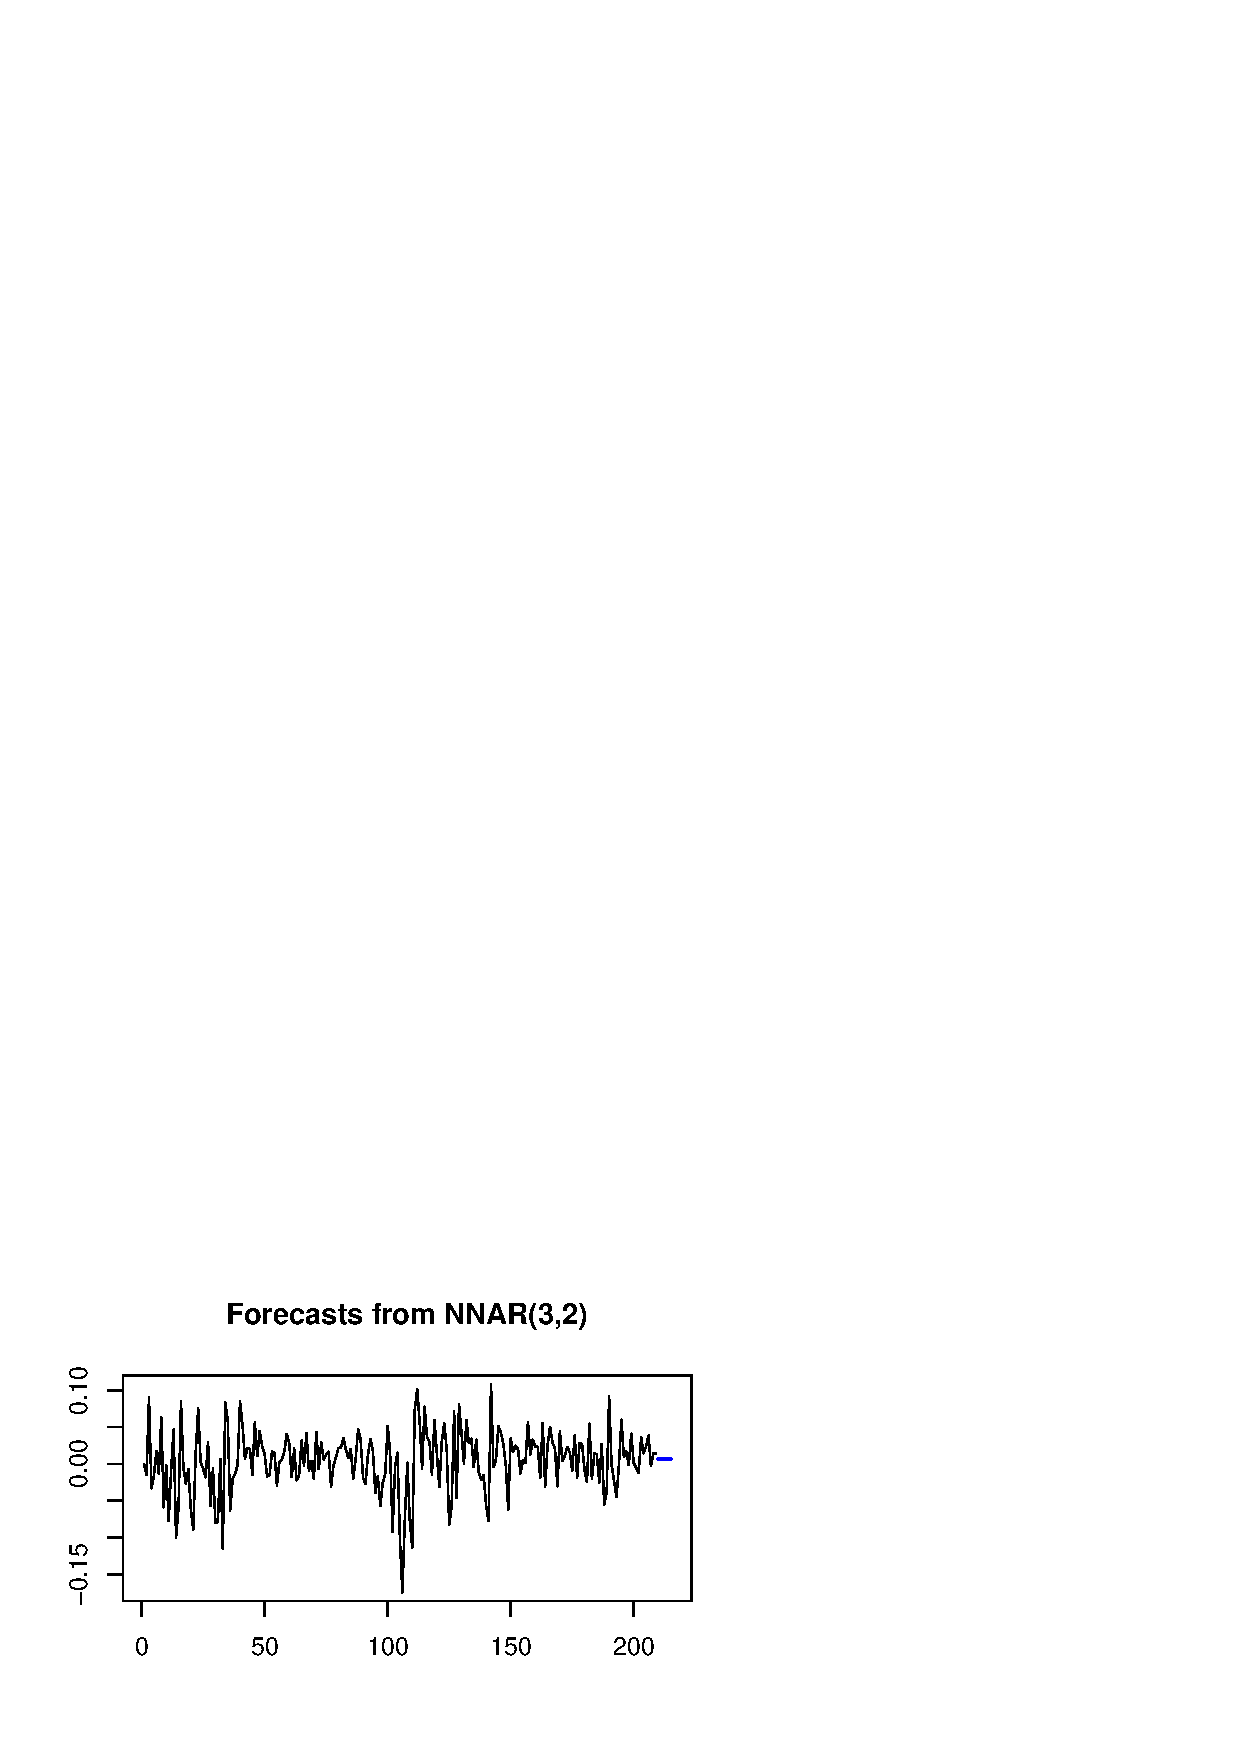
\includegraphics[scale=0.25]{nnar.pdf}
\end{figure}

\end{frame}

%---------------------------------------------------------
%---------------------Slide 27--------------------------
\begin{frame}
\frametitle{Feed forward neural network}
\textbf{Ejemplo 2 - Pronosticando el S$&$P 500} 

\vspace{4mm}	

Claramente para el per\'{i}odo 2000-2017 gana la rede neuronal autoregresiva, considerando las no-linealidades presentes.


\begin{figure}[t!]
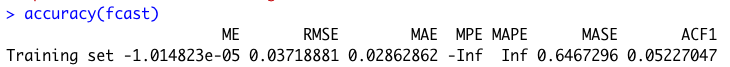
\includegraphics[scale=0.35]{ann.png}
\end{figure}

\begin{figure}[t!]
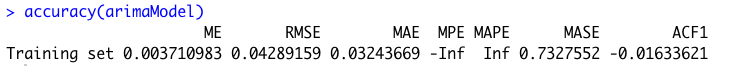
\includegraphics[scale=0.35]{arima.png}
\end{figure}

\end{frame}

%---------------------------------------------------------
%---------------------Slide 28--------------------------
\end{section}

\begin{section}{Support Vector Machines (SVM)}
\begin{frame}
\frametitle{Support Vector Machines (SVM)}
Fueron creadas por Boser, Guyon y Vapnik en 1992 \cite{boser1992training}. La formulaci\'on original esta motivada por la resoluci\'on de problemas de clasificaci\'on, donde la idea b\'asica consiste en \textbf{mapear los datos desde el espacio original a un espacio de mayor dimensi\'on a trav\'es de una transformaci\'on no lineal escogida a priori, para luego contruir el hiperplano de separaci\'on optimo en el nuevo espacio}. De esta manera, mediante la resoluci\'on de un problema lineal en el nuevo espacio, se tiene un modelo no lineal en el espacio original. 
\end{frame}
%---------------------------------------------------------
%---------------------Slide 29--------------------------
\begin{frame}
\frametitle{Support Vector Machines (SVM)}
En base a la misma filosof\'{i}a, el m\'etodo se extendi\'o luego a problemas de regresi\'on y de clustering. Desde su creaci\'on, SVM ha acaparado gran atenci\'on te\'orica, siendo aplicado con gran \'exito a problemas pr\'acticos de predicci\'on de series de tiempo de distinta naturaleza. \\
Dentro de las principales caracter\'{i}sticas de SVM se cuentan: i) la posibilidad de resolve un problema convexo, sin entrampamientos en \'optimos locales, ii) la representaci\'on de la soluci\'on en base a una fracci\'on del total de puntos disponibles (estos puntos son los llamados Support Vectors), iii) la capacidad de generalizaci\'on a nuevos datos, debido a que el algoritmo SVM se basa en el principio de minimizaci\'on del riesgo estructural propuesto en la Teor\'{i}a de Aprendizaje Estad\'{i}stico de Vapnik, y iv) la capacidad de modelar fen\'omenos no lineales mediante la ya mencionada transformaci\'on de los datos desde el espacio original a un espacio de mayor dimensi\'on, espacio en el cual se obtiene un modelo lineal que equivale a un modelo lineal en el espacio original.
\end{frame}
%---------------------------------------------------------
%---------------------Slide 30--------------------------
\begin{frame}
\frametitle{Support Vector Machines (SVM)}
En base a la misma filosof\'{i}a, el m\'etodo se extendi\'o luego a problemas de regresi\'on y de clustering. Desde su creaci\'on, SVM ha acaparado gran atenci\'on te\'orica, siendo aplicado con gran \'exito a problemas pr\'acticos de predicci\'on de series de tiempo de distinta naturaleza. \\
Dentro de las principales caracter\'{i}sticas de SVM se cuentan: i) la posibilidad de resolve un problema convexo, sin entrampamientos en \'optimos locales, ii) la representaci\'on de la soluci\'on en base a una fracci\'on del total de puntos disponibles (estos puntos son los llamados Support Vectors), iii) la capacidad de generalizaci\'on a nuevos datos, debido a que el algoritmo SVM se basa en el principio de minimizaci\'on del riesgo estructural propuesto en la Teor\'{i}a de Aprendizaje Estad\'{i}stico de Vapnik, y iv) la capacidad de modelar fen\'omenos no lineales mediante la ya mencionada transformaci\'on de los datos desde el espacio original a un espacio de mayor dimensi\'on, espacio en el cual se obtiene un modelo lineal que equivale a un modelo lineal en el espacio original.
\end{frame}
%---------------------------------------------------------
%---------------------Slide 31--------------------------
\begin{frame}
\frametitle{Support Vector Machines (SVM)}
\textbf{Defniciones del modelo - Funciones de Kernel}

Un kernel se definie como una funci\'on $K$, tal que $\forall x, y \epsilon K$

\begin{equation*} 
K(x,z) = < \Phi(x) \Phi (z) >
\end{equation*}

donde $X$ es el espacio de los datos de entrada (finito, generalmente $R^n$); y $\Phi$ es una funci\'on de mapeo de los datos de entrada desde $X$ a un espacio $F$ de mayor dimension, donde  $< \bullet , \bullet >$ es el producto interno de F. \\
Se puede probar que $K(x,z)$ es una funci\'on de kernel si y s\'olo si la matriz $M=(K(x_i , x_j))^n_{i , j=1}$ es semidefinida positiva. \\
Algunos de los kernels m\'as comunes son: \\
\begin{itemize}
  \item Lineal: $K(x,x') = <x,x'>$
  \item Polinomial: $K(x,x') = (<x,x'>+1)^d $ 
  \item RBF: $K(x,x') = exp ( - ||x - x' ||^2 / \sigma^2) $
\end{itemize}    

\end{frame}
%---------------------------------------------------------
%---------------------Slide 32--------------------------
\begin{frame}
\frametitle{Support Vector Machines (SVM)}
\textbf{Defniciones del modelo - Estructura de la SVM}

El modelo de SVM se puede ver como capas de nodos, en donde: \\
\begin{itemize}
  \item La primera capa consta de n nodos, que corresponden al vector de entrada 
  \item La segunda capa consta de N nodos, que es la transformaci\'on no lineal a base de support vectors 
  \item La tercera capa contiene 1 solo nodo, que es la predicci\'on 
  \item Cada capa se conecta de forma completa con la siguiente 
  \item Los nodos que llegan al nodo de output se ponderan por constantes, que son a determinar por el modelo, y luego se suman 
\end{itemize}    

\end{frame}
%---------------------------------------------------------
%---------------------Slide 33--------------------------
\begin{frame}
\frametitle{Support Vector Machines (SVM)}
\textbf{Defniciones del modelo - Estructura de la SVM}
 
Durante el proceso de aprendizaje, la primera capa selecciona las bases $K(xi; X)$, $i = 1, \dots, N$; dentro del conjunto de bases posbles, en tanto que la segunda capa construye una funci\'on lineal en el nuevo espacio, lo que es equivalente a encontrar un modelo no lineal en el espacio de entrada. Las N bases seleccionadas son aquellas inducidas por los puntos denominados Support Vectors. 

\end{frame}
%---------------------------------------------------------
%---------------------Slide 34--------------------------
\begin{frame}
\frametitle{Support Vector Machines (SVM)}
\textbf{Defniciones del modelo - Funciones de p\'erdida}
 
El modelo que se busca es de la forma $y = f(x) + e$, donde $f(x)$ es una funci\'on no lineal y $e$ el error. Luego, uno desea minimizar el valor de $y_i -  f(xi) =e$; para cada $i$, y para esto se usa una funci\'on de p\'erdida. Las m\'as comunes son
\begin{itemize}
  \item Cuadr\'atica: 
  \begin{equation*} 
   L(f(x),y) = (f(x)-y)^2
   \end{equation*}
  \item $\epsilon - sensible$: 
\begin{equation*} 
L(f(x),y,\epsilon) = \left\lbrace
\begin{array}{ll}
 0 & \textup{ si }| f(x) - y| < \epsilon \\
| f(x) - y| < \epsilon & \textup{ si } no
\end{array}
\right.
\end{equation*}
  \item Huber:  
\begin{equation*} 
L(f(x),y,\epsilon) = \left\lbrace
\begin{array}{ll}
\frac{1}{2}(f(x) - y)^2 & \textup{ si }| f(x) - y| < \mu \\
\mu| f(x) - y| - \frac{\mu^2} {2} & \textup{ si } no
\end{array}
\right.
\end{equation*}
\end{itemize}    

\end{frame}
%---------------------------------------------------------
%---------------------Slide 35--------------------------
\begin{frame}
\frametitle{Support Vector Machines (SVM)}
\textbf{Algoritmo de Regresi\'on SVM}
 
El problema de optimizaci\'on que encuentra los pesos del modelo, usando funci\'on de p\'erdida $\epsilon sensible$ es:

\begin{equation}\label{eq1}
  \begin{gathered}
    min \quad \frac{1}{2} \| w \|^2  \\  
    s.a. \quad y_i- < w, \Phi(x_i) > -b \le \epsilon \\
    -y_i+ < w, \Phi(x_i) > +b \geq \epsilon 
  \end{gathered}
\end{equation}

\end{frame}
%---------------------------------------------------------
%---------------------Slide 36--------------------------
\begin{frame}
\frametitle{Support Vector Machines (SVM)}
\textbf{Algoritmo de Regresi\'on SVM}

Dado que puede que no exista soluci\'on para el problema anterior, se suele reformular como:

\begin{equation}\label{eq1}
  \begin{gathered}
    min \quad \frac{1}{2} \| w \|^2 + C \sum_{i=1}^{l} (\zeta_i +  \zeta_i^*) \\  
    s.a. \quad y_i- < w, \Phi(x_i) > -b \le \epsilon + \zeta_i\\
    -y_i+ < w, \Phi(x_i) > +b \geq \epsilon + \zeta_i\\
    \zeta_i,  \zeta_i^* \ge 0, i = 1, 2, \dots l
  \end{gathered}
\end{equation}
 


\end{frame}
%---------------------------------------------------------
%---------------------Slide 37--------------------------
\begin{frame}
\frametitle{Support Vector Machines (SVM)}

El problema es que puede ser que no exista soluci\'on, por lo que se reformula como:
donde C es un par\'ametro a fijar, que representa el trade-off entre la complejidad y la exactitud del modelo, y el par\'ametro $\epsilon$ representa el rango de tolerancia a los errores en el modelo. Este problema tiene soluci\'on, y adem\'as es convexo, por lo que los m\'etodos de optimizaci\'on convergen bien a la soluci\'on, y el planteamiento del dual es bastante m\'as sencilla que el problema primal.\\
\vspace{4mm}	
Una vez encontrados los pesos w, entonces nuestro modelos es:
\begin{equation*} 
y = \sum_{i=1}^{N} w_i K(X_i,x)
\end{equation*}

\end{frame}
\end{section}

%---------------------------------------------------------
%---------------------Slide 38--------------------------
\begin{frame}
\frametitle{Feed forward neural network}
\textbf{Ejemplo 3 - Calculando el beta de Mastercard } 

\vspace{4mm}	

\only<1|handout:1>{
\begin{exampleblock}{C\'odigo en R}

\# load required library\\
rm(list=ls())\\
library(quantmod) \\
library(e1071)\\
library(dynlm) \\
library(forecast)\\
library(TTR)\\
library(tseries) \\
library(lmtest) \\

\end{exampleblock}
}

\end{frame}

%---------------------------------------------------------
%---------------------Slide 39--------------------------
\begin{frame}
\frametitle{Feed forward neural network}
\textbf{Ejemplo 3 - Calculando el beta de Mastercard } 

\vspace{4mm}	

\only<1|handout:1>{
\begin{exampleblock}{C\'odigo en R}

getSymbols(``SPY", from = ``2000-01-01", to = ``2017-12-01", src =  ``yahoo", adjust =  TRUE, periodicity = ``monthly")\\
Returns = diff(log(Ad(SPY)))\\
Returns[as.character(head(index(Ad(SPY)),1))] = 0\\

getSymbols(``MA", from = ``2000-01-01", to = ``2017-12-01", src =  ``yahoo", adjust =  TRUE, periodicity = ``monthly")\\
Returns = diff(log(Ad(MA)))\\
Returns[as.character(head(index(Ad(MA)),1))] = 0\\

\end{exampleblock}
}

\end{frame}

%---------------------------------------------------------
%---------------------Slide 40--------------------------
\begin{frame}
\frametitle{Feed forward neural network}
\textbf{Ejemplo 3 - Calculando el beta de Mastercard } 

\vspace{4mm}	

\only<1|handout:1>{
\begin{exampleblock}{C\'odigo en R}

Y$<-$Returns.MA\\
X$<-$Returns.SPY\\

rmse $<-$ function(error)\\
$\{$\\
  sqrt(mean(error$^$2))\\
$\}$\\


\# Create a linear regression model\\
model1 $<-$ lm(Y $\string{~}$ X)\\
print(model1)\\
coeftest(model1)\\
error1 $<-$ model1$\$$residuals  \\
predictionRMSE.OLS $<-$ rmse(error1)   \\

\end{exampleblock}
}

\end{frame}

%---------------------------------------------------------
%---------------------Slide 41--------------------------
\begin{frame}
\frametitle{Feed forward neural network}
\textbf{Ejemplo 3 - Calculando el beta de Mastercard } 

\vspace{4mm}	

\only<1|handout:1>{
\begin{exampleblock}{C\'odigo en R}


\# Create a SVM regression model\\
model2 $<-$ svm(Y $\string{~}$ X)\\
print(model2)\\
error2 $<-$ model2$\$$residuals  \\
predictionRMSE.SVM $<-$ rmse(error2)   \\

\vspace{4mm}	

Para el timespam 2007-2012 tenemos:\\
predictionRMSE.OLS \tab
[1] 0.08724145\\
predictionRMSE.SVM \tab
[2] 0.08654265\\

\vspace{4mm}	

Sin embargo, para el timespam 2012-2017 tenemos:\\

predictionRMSE.OLS \tab
[1] 0.03777724\\
predictionRMSE.SVM \tab
[2] 0.03829508\\

\end{exampleblock}
}

\end{frame}

%---------------------------------------------------------
%---------------------Slide 42--------------------------
\begin{frame}
\frametitle{Feed forward neural network}
\textbf{Ejemplo 3 - Calculando el beta de Mastercard } 

\begin{figure}[t!]
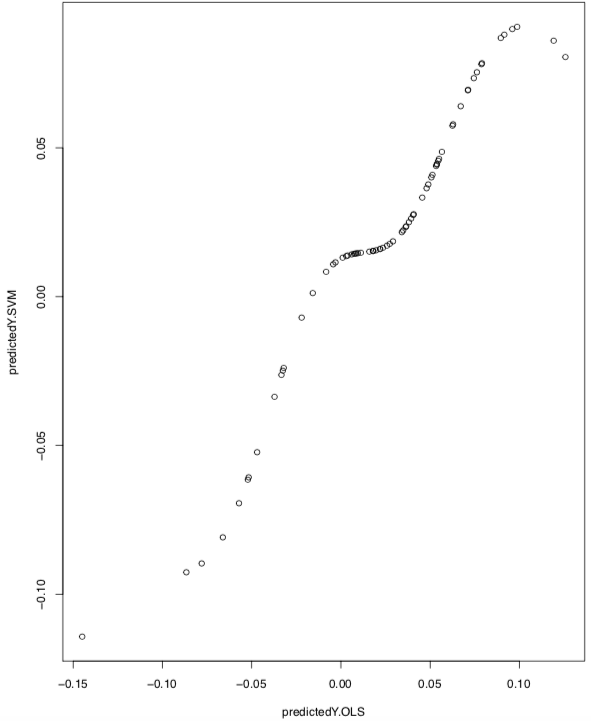
\includegraphics[scale=0.25]{svm_versus_ols.pdf}
\end{figure}

\end{frame}

%---------------------------------------------------------

%--------------Slide Referencias---------------------

\section{Referencias}
\begin{frame}[allowframebreaks]
        \frametitle{Referencias}
        \bibliographystyle{unsrt}
        \nocite{} %lista sin citar.
        \bibliography{TS_ref}
\end{frame}

%---------------------------------------------------------
%---------------------------------------------------------
\end{document} 
%---------------------------------------------------------




